\chapter{Evaluation}

\section{Measures of Success}

The success of the project can be measured by comparing the project results with objectives. We will also review the design choices in constructing the tool. The review will highlight the practical outcomes from using argumentation to explain scheduling.
\linespace
Arguably, the most important outcome of this project is that the tool is functionality correct. This means the tool is required to explain schedules for feasibility, efficiency and satisfaction with respect to user decisions.
\linespace
One objective is to implement an accessible tool. To measure accessibility, we can refer to the tractability complexity from explanations. The length of explanations either in the number of words or characters may be correlated with understandability. Alternatively, we can conduct a survey targeted towards potential users. Because the understandability of explanations are difficult to measure, we will attempt to quantity this using multiple choice questions. To carefully evaluate explanations, one would need to refer to cognitive science, which is beyond the scope of this project. In addition, we can measure performance to reflect responsiveness and scalability of the tool. This may be achieved by using profiling utilities to measure performance metrics such as time to generate explanations and memory consumption.
\linespace
We can also use the survey to ask how well our tool performs with respect to applicability and knowledge transfer. We can also infer the practical limitations from the tool to measure the applicability.

\section{Theoretical Results}

At the end of the project, we aim to present extensions of argumentation with scheduling We will explain the practicability of using argumentation Such details are open-ended.

\begin{figure}
	\begin{tabular}{lccc}
		\hline
		Algorithm & Computational & Memory & Tractability\\
		\hline
		\textsc{Construct-Feasibility} & $\mathcal{O}(m^2n^2)$ & $\mathcal{O}(m^2n^2)$ &\\
		\textsc{Construct-Efficiency} & $\mathcal{O}(m^2n^2)$ & $\mathcal{O}(m^2n^2)$ &\\
		\textsc{Construct-Satisfaction} & $\mathcal{O}(m^2n)$ & $\mathcal{O}(m^2n^2)$ &\\
		\textsc{Compute-Unattacked} & $\mathcal{O}(m^2n^2)$ & $\mathcal{O}(mn)$ &\\
		\textsc{Compute-Partial-Conflicts} & $\mathcal{O}(mn)$ & $\mathcal{O}(mn)$ &\\
		\textsc{Explain-Stability} & $\mathcal{O}(m^2n^2)$ & $\mathcal{O}(m^2n^2)$ &\\
		\textsc{Explain-Feasibility} & $\mathcal{O}(mn^2)$ & $\mathcal{O}(mn)$ & $\mathcal{O}(mn)$\\
		\textsc{Explain-Efficiency} & $\mathcal{O}(mn^2\log(mn))$ & $\mathcal{O}(mn^2)$ & $\mathcal{O}(mn^2)$\\
		\textsc{Explain-Satisfaction} & $\mathcal{O}(mn)$ & $\mathcal{O}(mn)$ & $\mathcal{O}(mn)$\\
		\textsc{Full-Precomputation-Explain} & $\mathcal{O}(m^2n^2\log n)$ & $\mathcal{O}(m^2n^2)$ & $\mathcal{O}(mn^2)$\\
		\textsc{Partial-Precomputation-Explain} & $\mathcal{O}(m^2n^2\log n)$ & $\mathcal{O}(mn^2)$ & $\mathcal{O}(mn^2)$\\
		\hline
	\end{tabular}
	\caption{Computational, memory and tractability complexity of algorithms}
\end{figure}

\section{Practical Results} 

I will be able to demonstrate the tool, and its functionality. This will be reflected in the report through a user documentation guide.

\subsection{Full versus Partial Precomputation}

We will compare two algorithmic approaches to AAF construction. The algorithms are implemented, then profiled for elapsed time and maximum allocated memory. The time and memory are measured with the Python's \texttt{cProfile} and \texttt{memory-profiler} modules respectively. The tool was executed on Department of Computing's virtual machines, with the specification of 2 core CPU at 2GHz with 2GB RAM.
\linespace
Time comparison:
\begin{itemize}
	\item Elapsed time measurements are noisy.
	\item For less than 100 jobs, both approaches have approximately equal timings.
	\item From profiling, the tool takes 0.7 seconds to startup.
	\item Partial precomputation is 26\% slower than full precomputation on average from the samples illustrated on the graph, excluding startup time.
	\item Both graphs hints at quadratic complexity.
\end{itemize}

Memory comparison:
\begin{itemize}
	\item For less than 40 jobs, both approaches have approximately equal memory usage.
	\item From profiling, the tool uses 72MiB to startup.
	\item For a large number of jobs, partial-precomputation is 18 times more efficient than full precomputation excluding startup memory.
	\item Both graphs hints at quadratic complexity.
\end{itemize}

\newpage

\begin{figure}[H]
	\centering
	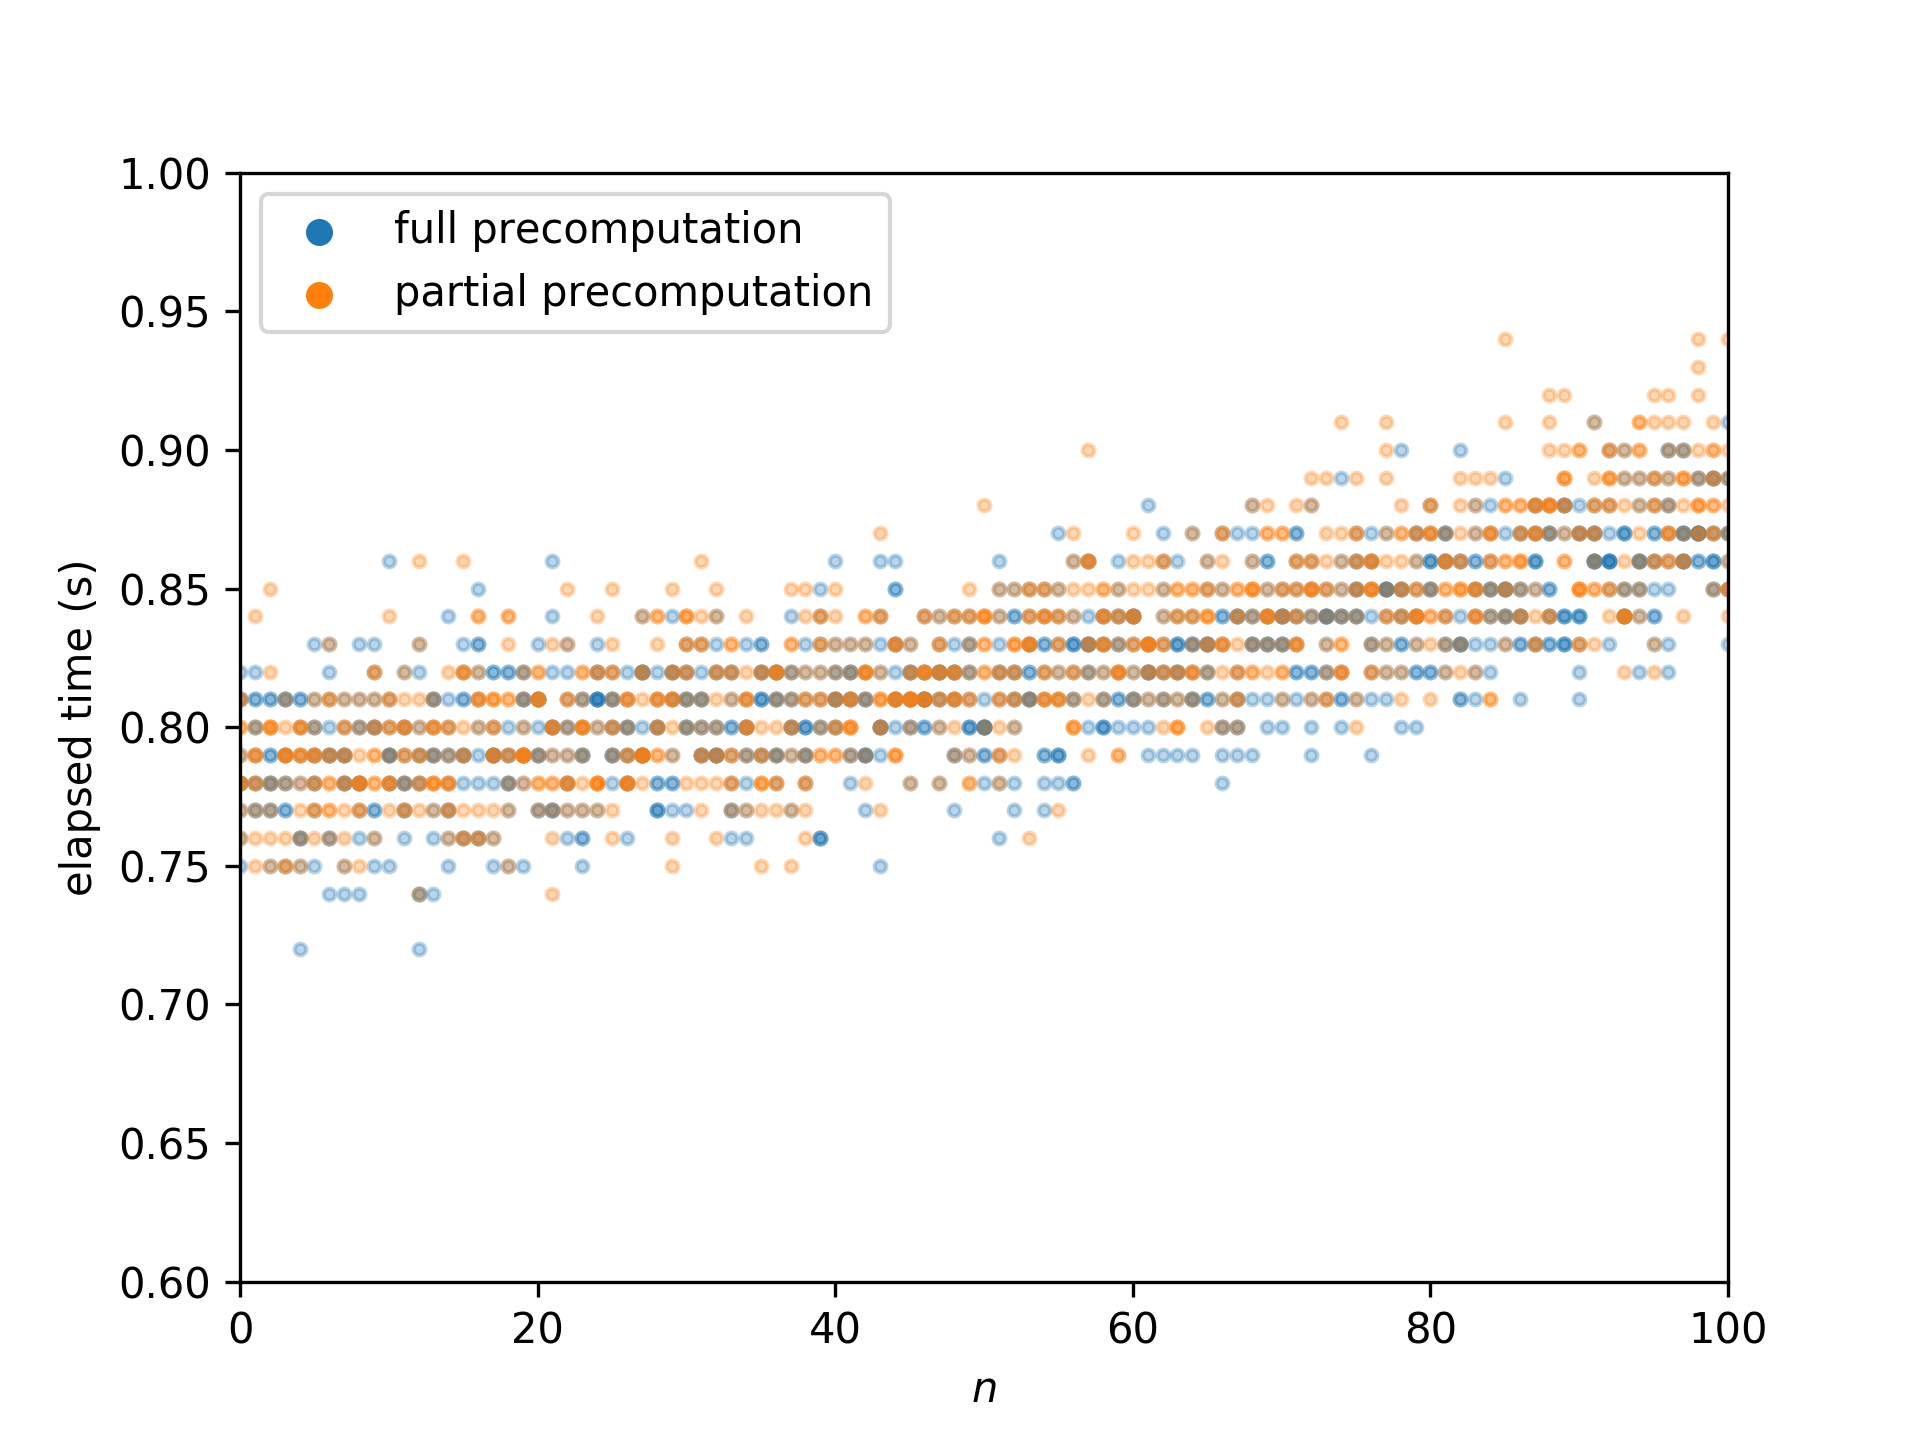
\includegraphics[scale=0.7]{figures/precomputation_cpu_small}
	\caption{Elapsed time comparison where $m=10$ and $0\leq n\leq 100$ with 1000 samples.}
\end{figure}

\begin{figure}[H]
	\centering
	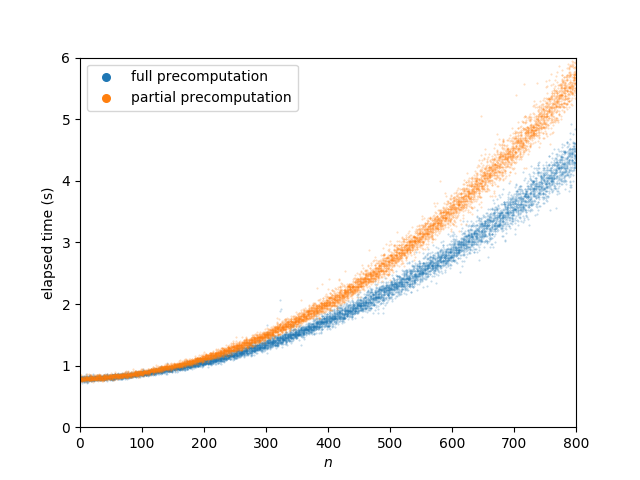
\includegraphics[scale=0.7]{figures/precomputation_cpu_big}
	\caption{Elapsed time comparison where $m=10$ and $0\leq n\leq 800$ with 8000 samples.}
\end{figure}

\begin{figure}[H]
	\centering
	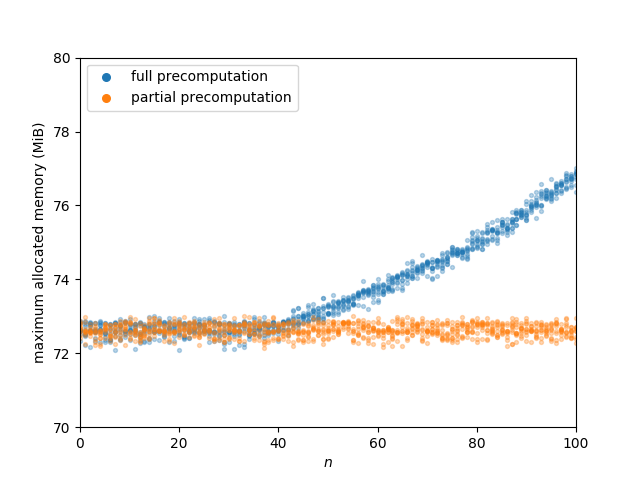
\includegraphics[scale=0.7]{figures/precomputation_memory_small}
	\caption{Maximum allocated memory comparison where $m=10$ and $0\leq n\leq 100$ with 1000 samples.}
\end{figure}

\begin{figure}[H]
	\centering
	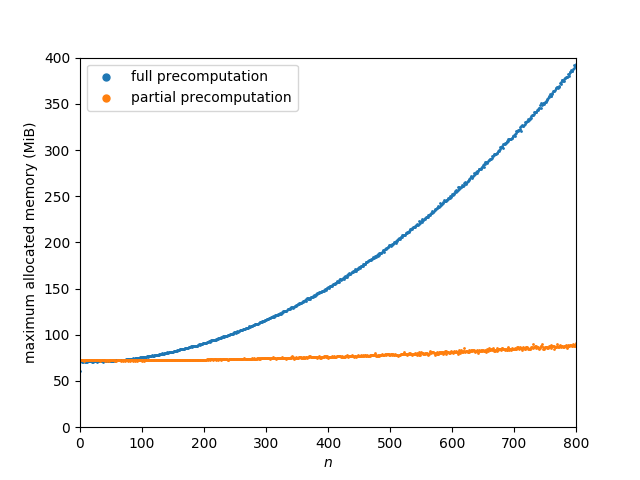
\includegraphics[scale=0.7]{figures/precomputation_memory_big}
	\caption{Maximum allocated memory comparison where $m=10$ and $0\leq n\leq 800$ with 8000 samples.}
\end{figure}